\newpage
\section{Auswertung}
\subsection{Effektiver Dämpfungswiderstand und Abklingdauer}
\begin{figure}
    \centering
    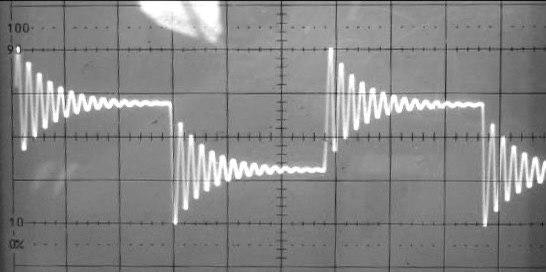
\includegraphics[width=0.7\textwidth]{bilder/Bild_5a_screen.jpg}
    \caption{
        Gemessene Kondensatorspannung bei einem RCL-Kreis mit angelegter Rechteckspannung. 
        Mit t $20\mu s/Div.$ und V $ 2V/Div.$
        }
    \label{fig:bild1}
\end{figure}

\begin{table}
    \centering
    \begin{tabular}{c c}
        \toprule
        $U(t)\;/\;2V$ & $t\;/\;20\mu s$\\
        \midrule
        2.0     &0   \\
        1.6     &0.25\\
        1.4     &0.45\\
        1.25    &0.6\\
        1.1     &0.9\\
        1.05    &1.0\\
        1.0     &1.2\\
        0.9     &1.4\\
        0.8     &1.6\\
        0.78    &1.8\\
        \bottomrule
    \end{tabular}
    \caption{Amplituden aus gedämpften Schwingkries gegenüber der Zeit}
    \label{tab:tabelle1}
\end{table}

Mit dem Widerstand $R1=(30.3\pm0.01)\si{\ohm}$, der Induktivität $L=(3.5 \pm 0.01)mH$ der Schaltung und $y_0=4V$ folgt die Theoriekurve
\begin{align}
    y(t)&=4 \cdot e^{-R/2L \cdot t}\\
    y(t)&\approx 4 \cdot e^{-(4.33\pm0.01) \cdot 10^3*t}
\end{align}
\newpage
Insgesamt ergibt sie somit für die Messdaten und dessen Ausgleichsfunktion $y(t)=e^{-k*t}$
sowie für die Theoriekurve
\begin{figure}
    \centering
    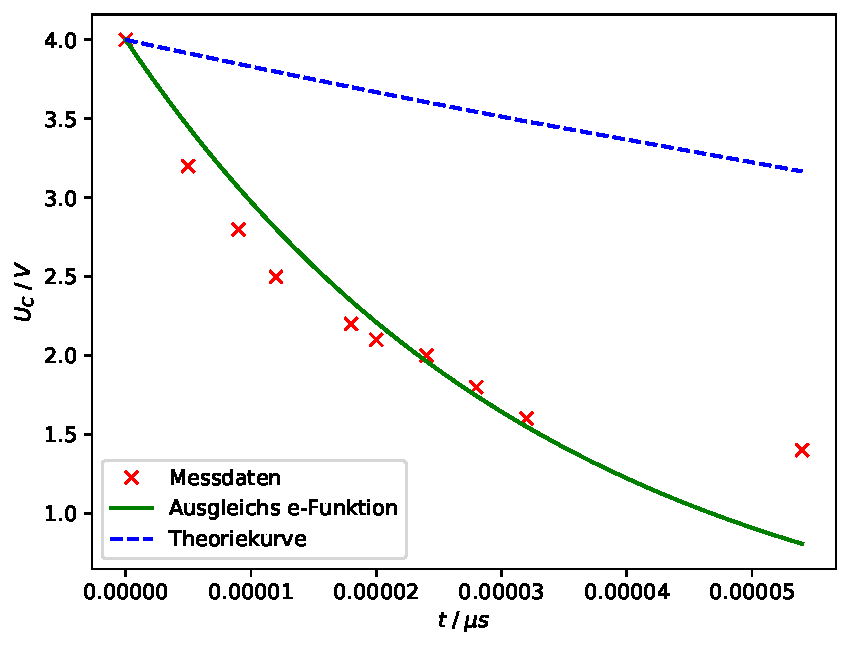
\includegraphics[width=0.7\textwidth]{bilder/plota.pdf}
    \caption{
        Darstellung der Daten der einhüllenden der gedämpften Schwingungen mit ihrer
        Ausgleichsfunktion $y(t)\approx 4 \cdot e^{-3.08\cdot10^4 \cdot t}$ verglichen mit der Theoriekurve
    }
    \label{fig:ultra_plot}
\end{figure}
aus den Daten und der Ausgleichsfunktion folgt somit der effektive Dämpfungswiderstand 
$R_{eff}$
\begin{equation}
    R_{eff}= 3.08\cdot10^4 \cdot 2L \approx 215\si{\ohm}
\end{equation}
Die Abklingdauer $T_{ex}$ ergibt sich somit
\begin{equation}
    T_{ex}=\frac{2L}{R_{eff}}\approx 3.25 \cdot 10^{-4}s
\end{equation}
\label{sec:Auswertung}

\subsection{Aperiodischer Grenzfall}
Der Spezialfall liefert:
\begin{equation}
    R_{ap}=\sqrt{\frac{4L}{C}}=1673.32\si{\ohm}     %fehler und Fehlerrechnung fehlt
\end{equation}
\subsection{}


